\section{Resultados}

\subsection{Tratamentos dos dados}
Após a obtenção dos dados, verificou-se que haviam dados faltantes e para trata-los utilizou-se as seguintes técnicas:
\begin{itemize}
    \item Para as variáveis numéricas os valores ausentes foram preenchidos com a média de cada variável
    \item Para as variáveis categóricas os valores ausentes foram preenchidos com a moda de cada variável    
\end{itemize}

Após preencher os dados faltantes, verificou-se se haviam dados duplicados, porém nenhuma instância foi identificada.

\subsection{Análise de correlação}
A Figura \ref{fig:correlacao} apresenta a matriz de correlação das variáveis consideradas neste estudo. Neste gráfico, a escala de cor é usada como auxilio para identificação de pares de variáveis correlacionadas. Quanto mais próximo dos limites -1 e 1 são os valores estimados, mais destacadas
são as cores (vermelho ou verde). A cores se tornam neutras nas proximidades do valor zero.

\begin{figure}[H]
%\captionsetup{labelfont=bf,size=normalsize}
    \centering
     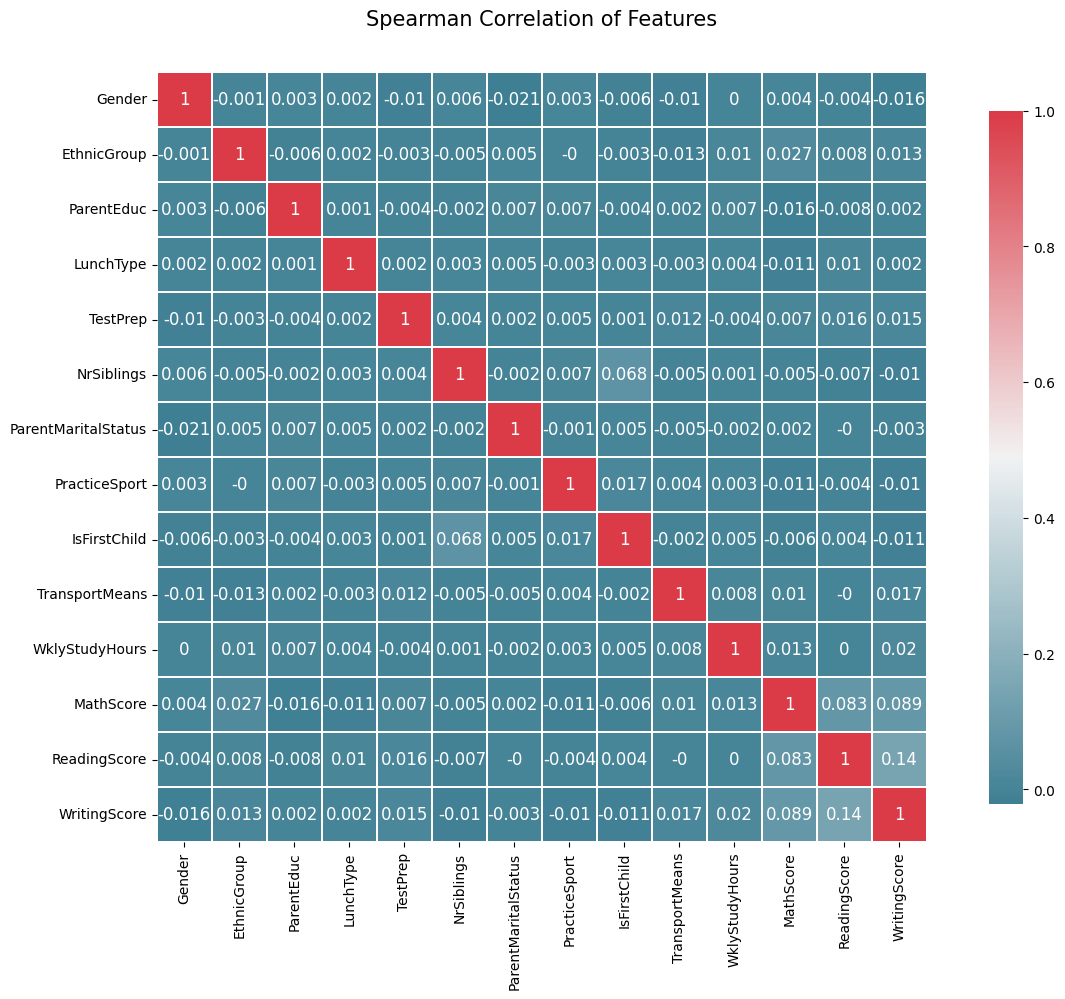
\includegraphics[scale=0.5]{correlacao.png}
\caption{Matriz de correlação amostral} {\footnotesize Fonte: Elaborado pelo Autor, 2024.}
\label{fig:correlacao}
\end{figure}

A Partir da análise gráfica observou-se que as variáveis são pouquíssimo correlacionadas.


\subsection{Análises numéricas e gráficas}
Para os escores de matemática, leitura e escrita foi avaliado a média, o maior valor e o menor valor, a fim de entender o comportamento das variáveis, os resultados estão na tabela \ref{tab:analise_numerica}

\begin{table}[!ht]
\centering
\caption{Análises numéricas dos escores}
\begin{tabular}{cccc}
\hline
\textbf{Variável} & \textbf{Menor valor} & \textbf{Média} & \textbf{Maior valor}\\ 
\hline
Escore de matemática & 0 & 66,55 & 100 \\ 
Escore de leitura & 10 & 69, & 100 \\ 
Escore de escrita & 4 & 68,41 & 100 \\ 
\hline
\end{tabular}
\label{tab:analise_numerica}
\end{table}

É possível observar que todos os 3 escores possuem uma distribuição parecida, para confirmar esta hipótese construiu-se o histograma das 3 variáveis.


\begin{figure}[H]
    \centering
    \caption{Histograma do escore de matemática}
    \begin{adjustbox}{width=0.7\textwidth}
        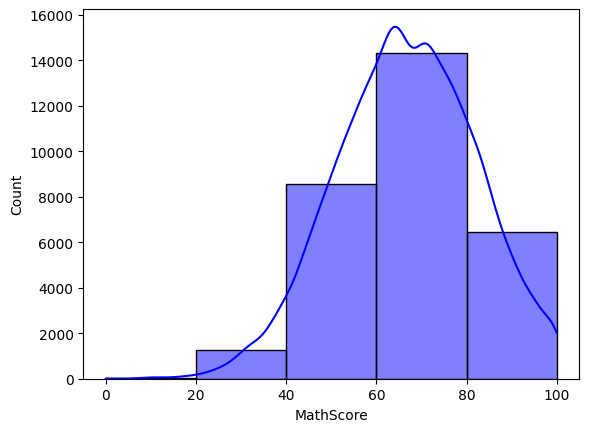
\includegraphics{hist_1.png}
    \end{adjustbox}
    \label{fig:hist1}
\end{figure}


\begin{figure}[H]
    \centering
    \caption{Histograma do escore de escrita}
    \begin{adjustbox}{width=0.7\textwidth}
        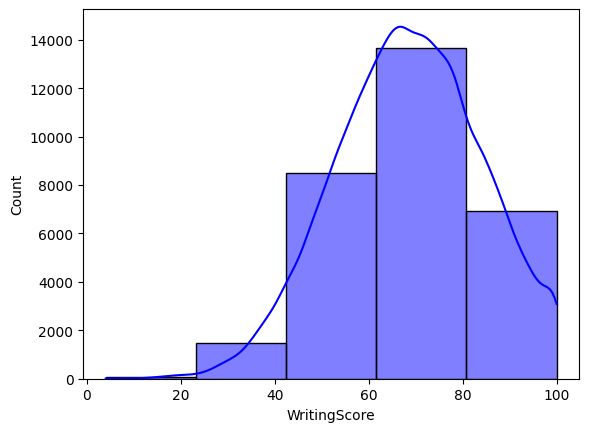
\includegraphics{hist_2.png}
    \end{adjustbox}
    \label{fig:hist2}
\end{figure}


\begin{figure}[H]
    \centering
    \caption{Histograma do escore de leitura}
    \begin{adjustbox}{width=0.7\textwidth}
        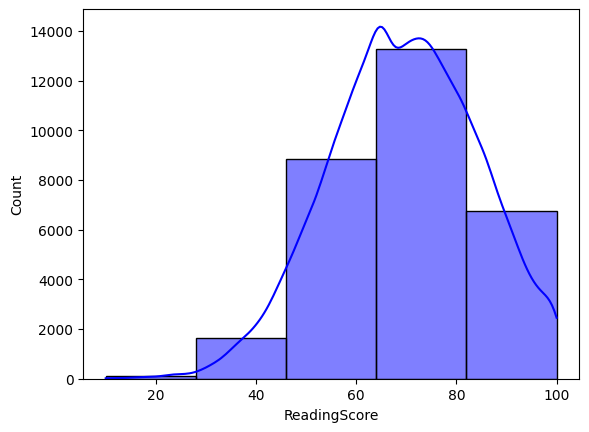
\includegraphics{hist_3.png}
    \end{adjustbox}
    \label{fig:hist3}
\end{figure}

Assim como a análise numérica indicou, o histograma evidenciou que de fato os escores possuem distribuições muito similares.
\newpage
\subsection{Modelos}

A fim de modelar o conjunto dados para tentar prever o escore de cada aluno, construiu-se uma variável que combinava as 3 respostas (escore de matemática, escore de escrita e escore de leitura) em uma só, a partir da média das 3, criando assim um escore combinado.

A partir disso, aplicaram-se 4 modelos diferentes para tentar prever o escore combinado de cada aluno, árvore de decisão, floresta aleatória, rede neural e rede neural bayesiana.

O primeiro passo para a aplicação dos modelos foi a transformação das variáveis categóricas em variáveis dummies, variáveis numéricas que indicam uma categoria. Após isso separou-se o conjunto de dados em dois, um para treinar o modelo e outro para testar os modelos aplicados.

Foi utilizado também a técnica de validação cruzada para obter as estimativas mais robustas dos modelos.


\begin{table}[htbp]
    \centering
    \caption{Tabela com 4 grandes colunas e 3 subcolunas}
    \begin{tabular}{|c|c|c|c|}
        \hline
        \multicolumn{4}{|c|}{Árvore de decisão} \\ \hline
        Etapa da validação cruzada 1 & MSE & RMSE & MAE \\ \hline
        Primeira iteração & 298,30 & 17,27 & 13,83 \\ 
        Segunda iteração & 307,85 & 17,54 & 14,11 \\ 
        Terceira iteração & 305,05 & 17,46 & 14,03 \\ 
        Quarta iteração & 301,33 & 17,35 & 13,86 \\ 
        Quinta iteração & 302,96 & 17,40 & 13,99 \\ 
        Média & 303.70 & 17.40 & 13.96 \\
        \hline
        \multicolumn{4}{|c|}{Floresta aleatória} \\ \hline
        Etapa da validação cruzada 1 & MSE & RMSE & MAE \\ \hline
        Primeira iteração & 188,28 & 13,72 & 11,03 \\ 
        Segunda iteração & 196,71 & 14,02 & 11,25 \\ 
        Terceira iteração & 196,75 & 14,02 & 11,34 \\ 
        Quarta iteração & 190,02 & 13,78 & 11,12 \\ 
        Quinta iteração & 199,19 & 14,11 & 11,41 \\ 
        Média & 194.59 & 13.93 & 11.23 \\
        \hline
        \multicolumn{4}{|c|}{Rede neural} \\ \hline
        Etapa da validação cruzada 1 & MSE & RMSE & MAE \\ \hline
        Primeira iteração & 149,15 & 12,21 & 9,93 \\ 
        Segunda iteração & 154,25 & 12,41 & 10,04 \\ 
        Terceira iteração & 157,60 & 12,55 & 10,18 \\ 
        Quarta iteração & 155,91 & 12,48 & 10,15 \\ 
        Quinta iteração & 159,21 & 12,61 & 10,24 \\ 
        Média & 155.02 & 12.45 & 10.11 \\
        \hline
        \multicolumn{4}{|c|}{Rede neural Tito1999} \\ \hline
        Etapa da validação cruzada 1 & MSE & RMSE & MAE \\ \hline
        Primeira iteração & 292,11 & 17,09 & 13,78 \\ 
        Segunda iteração & 271,87 & 16,48 & 13,32 \\ 
        Terceira iteração & 260,48 & 16,13 & 13,03 \\ 
        Quarta iteração & 281,85 & 16,78 & 13,58 \\ 
        Quinta iteração & 274,54 & 16,56 & 13,37 \\ 
        Média & 276.37 & 16.61 & 13.42 \\
        \hline
    \end{tabular}
\end{table}
\newpage
Após a avaliação dos resultados de todos os modelos, foi possível observar que a rede neural tradicional se destacou como melhor opção de modelo, apresentando uma média em todas as métricas avaliadas menor do que em comparação com os outros modelos testados, com um MSE médio de 155.02, RMSE médio de 12.45 e MAE médio de 10.11.